\documentclass[12pt]{article}
\usepackage{{../preamble}}
\graphicspath{{pics}}

\begin{document}
\chead{Problem Set 3}

%%%%%%%%%%%%%%%%%%%%%%%%%%%%%%%%%%%%%%%%%%%%%%%
%                  Definitions                %
%%%%%%%%%%%%%%%%%%%%%%%%%%%%%%%%%%%%%%%%%%%%%%%
\def\xdot{\dot X} \def\ydot{\dot Y} \def\zdot{\dot Z}
\def\kdot{\dot k} \def\ccdot{\dot c} \def\ddt{\frac{d}{dt}}
\def\dfdk{\frac{\partial F}{\partial K}}
\def\dfdl{\frac{\partial F}{\partial L}}
\def\plim{\lim\limits_{\phi\to 0}}
\def\ddp{\dfrac{\partial}{\partial \phi}}
\def\dgdp{\dfrac{\partial\gamma}{\partial \phi}}
\def\invphi{\sfrac{1}{\phi}}
\def\kone{k^*_1} \def\ktwo{k^*_2}




%%%%%%%%%%%%%%%%%%%%%%%%%%%%%%%%%%%%%%%%%%%%%%%
%                Problem 1                    %
%%%%%%%%%%%%%%%%%%%%%%%%%%%%%%%%%%%%%%%%%%%%%%%
\section*{Problem 1}
\problem{The elasticity of substitution with constant-relative-risk-aversion utility: Romer 2.2}{
    Consider an individual who lives for two periods and whose utility is given by equation (2.43). Let $P_1$ and $P_2$ denote the prices of consumption in the two periods, and let $W$ denote the value of the individual’s lifetime income; thus the budget constraint is $P_1C_1 + P_2C_2 = W$.

    \begin{enumerate}[label=(\alph*)]
    \item What are the individual’s utility-maximizing choices of $C_1$ and $C_2$, given $P_1$, $P_2$, and $W$?
    \end{enumerate} 
}


\def\cone{\frac{C_{1t}^{1-\theta}}{1-\theta}}
\def\ctwo{\frac{1}{1+\rho}\frac{C_{2(t+1)}^{1-\theta}}{1-\theta}}
\begin{align*}
\intertext{The Lagrangian for this problem is}
\L &= U(t) + \lambda (W - P_1C_1 - P_2C_2) \\[1em]
    &= \cone + \ctwo + \lambda (W - P_1C_1 - P_2C_2) \\[1em]
\intertext{Supressing the $t$ subscript, we the FOCs are}
\part{\L}{C_1} &= 0 \implies \frac{1}{\lambda} = P_1 C_1^\theta \\[1em]
\part{\L}{C_2} &= 0 \implies \frac{1}{\lambda} = P_2 C_2^\theta (1+\rho) \\[1em]
\intertext{So}
P_1 C_1^\theta &= P_2 C_2^\theta (1+\rho) \\[1em]
C_1 &= C_2\l[\frac{P_2}{P_1}(1+\rho)\r]^{1/\theta}
\intertext{Plugging this into the budget constraint...}
W &= P_1C_1 + P_2C_2 \\[1em]
    &= P_1C_2\l[\frac{P_2}{P_1}(1+\rho)\r]^{1/\theta} + P_2C_2 \\[1em]
    &= P_2C_2\l\{\l[\l(\frac{P_1}{P_2}\r)^{\theta-1}(1+\rho)\r]^{1/\theta} + 1\r\} \\[1em]
\intertext{So the optimal period 2 consumption is}
C_2^* &= \frac{W}{ P_2\l\{\l[\l(\frac{P_1}{P_2}\r)^{\theta-1}(1+\rho)\r]^{1/\theta} + 1\r\}}
\intertext{And the optimal period 1 consumption is}
C_1^* &= C_2^*\l[\frac{P_2}{P_1}(1+\rho)\r]^{1/\theta} \\[1em]
    &= \frac{W\l[\frac{P_2}{P_1}(1+\rho)\r]^{1/\theta}}{ P_2\l\{\l[\l(\frac{P_1}{P_2}\r)^{\theta-1}(1+\rho)\r]^{1/\theta} + 1\r\}}
\intertext{Which probably simplifies...}
\end{align*}



%%%%%%%%%%%%%%%%%
%     Part b    %
%%%%%%%%%%%%%%%%%
\newpage\problem{}{
    \begin{enumerate}[label=(\alph*)]
    \setcounter{enumi}{1}
    \item The elasticity of substitution between consumption in the two periods is
$-[(P_1/P_2)/(C_1/C_2)][\partial(C_1/C_2)/\partial(P_1/P_2)]$, or $-\partial \ln (C_1/C_2)/\partial \ln (P_1/P_2)$. Show that
with the utility function (2.43), the elasticity of substitution between $C_1$ and
$C_2$ is $1/\theta$.
    \end{enumerate} 
}


\begin{align*}
\intertext{Since we know that}
\frac{C_1^*}{C_2^*} &= \l[\frac{P_2}{P_1}(1+\rho)\r]^{1/\theta}
\intertext{Then}
\ln\frac{C_1^*}{C_2^*} &= \frac{1}{\theta}\ln\l[\frac{P_2}{P_1}(1+\rho)\r] \\[1em]
    &=\frac{1}{\theta}\l[\ln(1+\rho) - \ln\frac{P_1}{P_2} \r]
\intertext{So}
\part{\ln\dfrac{C_1^*}{C_2^*}}{\ln\dfrac{P_1}{P_2}}
    &= -\frac{1}{\theta}
\end{align*}





%%%%%%%%%%%%%%%%%%%%%%%%%%%%%%%%%%%%%%%%%%%%%%%
%                Problem 2                    %
%%%%%%%%%%%%%%%%%%%%%%%%%%%%%%%%%%%%%%%%%%%%%%%
\newpage
\section*{Problem 2}
\problem{Find the utility-maximizing path of $C$: Romer 2.5}{
    Consider a household with utility given by (2.2) (2.3). Assume that the real interest
rate is constant, and let $W$ denote the household’s initial wealth plus the present
value of its lifetime labor income (the right-hand side of [2.7]). Find the utility-maximizing path of $C$, given $r$, $W$, and the parameters of the utility function.
}

\def\ut{\frac{C(t)^{1-\theta}}{1-\theta}}
\def\lh{\frac{L(t)}{H}}
\def\lt{\lambda(t)}
\def\ldot{\dot\lambda}
\begin{align*}
\intertext{First note that since $r(t)=r$ is a constant, }
R(t) &= \int_0^tr(s)dt = \int_0^trdt = rt
\intertext{so the path of consumption satisfies}
\argmax_{C(t)} & \int_0^\infty e^{-\rho t}\ut\lh dt
\intertext{subject to the conditions}
    & \int_0^\infty e^{-rt}C(t)\lh dt \leq W\\[1em]
    & \kdot = f(k) - C - (n+g)k \\[1em]
    & f'(k) = r(t) = r
\intertext{So the Hamiltonian for this problem is}
H &= e^{-\rho t}\ut\lh + \lt
    \l[f(k(t)) - C(t) - (n+g)k(t)\r]
\intertext{And the first FONC is}
H_C = 0 &\implies \lt = e^{-\rho t}C(t)^{-\theta}\lh
\intertext{taking logs and then the time derivative gives}
    &\implies \ln\lt = -\rho t -\theta\ln C(t) + \ln L - \ln H \\[1em]
    &\implies \frac{\ldot}{\lambda} = -\rho -\theta\frac{\dot C}{C}+\frac{\dot L}{L}
\intertext{And noting that the growth rate of labor is $n$}
    &\implies \frac{\ldot}{\lambda} = -\rho -\theta\frac{\dot C}{C}+n
\intertext{Then the second FONC is}
H_k = -\ldot &\implies -\frac{\ldot}{\lambda} = f'(k) - (n+g)
\intertext{And noting that $f'(k)=r(t)=r$,}
    &\implies -\frac{\ldot}{\lambda} = r - n -g
\intertext{Putting these first two FONCs together, we have}
r - n -g &= \rho +\theta\frac{\dot C}{C} -n \\[1em]
\frac{\dot C}{C} &= \frac{1}{\theta}(r-g-\rho)
\intertext{Since this is a constant, this implies that}
C(t) &= Ae^{-\frac{1}{\theta}(g+\rho-r)}
\intertext{For some constant $A$ determined by the initial capital stock $k_0$ and the law of motion $\kdot = f(k)-C(t)-(n+g)k$.}
\end{align*}










%%%%%%%%%%%%%%%%%%%%%%%%%%%%%%%%%%%%%%%%%%%%%%%
%                Problem 3                    %
%%%%%%%%%%%%%%%%%%%%%%%%%%%%%%%%%%%%%%%%%%%%%%%
\newpage
\section*{Problem 3}
\problem{Using the phase diagram to analyze the impact of an anticipated change: Romer 2.11}{
    Consider the policy described in Problem 2.10, but suppose that instead of announcing and implementing the tax at time 0, the government announces at time 0 that at some later time, time $t_1$, investment income will begin to be taxed at rate $\tau$.

    \begin{enumerate}[label=(\alph*)]
        \item Draw the phase diagram showing the dynamics of $c$ and $k$ after time $t_1$.
    \end{enumerate} 
}
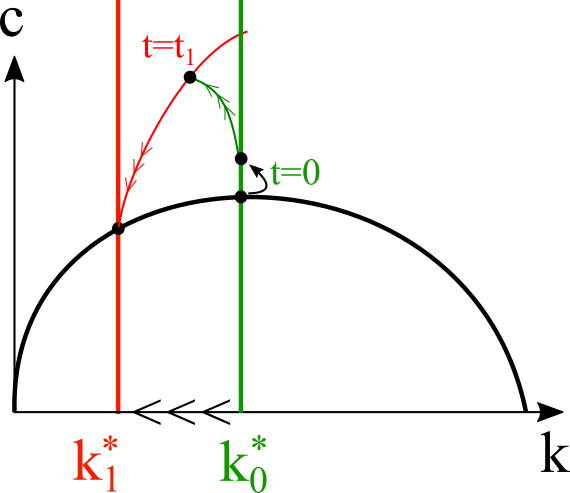
\includegraphics[width=0.8\textwidth]{3.a}



%%%%%%%%%%%%%%%%%
%     Part b    %
%%%%%%%%%%%%%%%%%
\newpage\problem{}{
    \begin{enumerate}[label=(\alph*)]
    \setcounter{enumi}{1}
    \item Can $c$ change discontinuously at time $t_1$? Why or why not?
    \end{enumerate} 
}
No, if $c$ changed discontinuously at $t_1$, that would indicate that the consumers were not consumption smoothing before $t_1$ even though they had know about the change in tax rate since $t=0$. So, right before $t_1$, $c$ must be approaching the new value it will have at the time of the tax change $t_1$.



%%%%%%%%%%%%%%%%%
%     Part c    %
 %%%%%%%%%%%%%%%%% \newpage
\newpage
\problem{}{
    \begin{enumerate}[label=(\alph*)]
    \setcounter{enumi}{2}
    \item Draw the phase diagram showing the dynamics of $c$ and $k$ before $t_1$.
    \end{enumerate} 
}

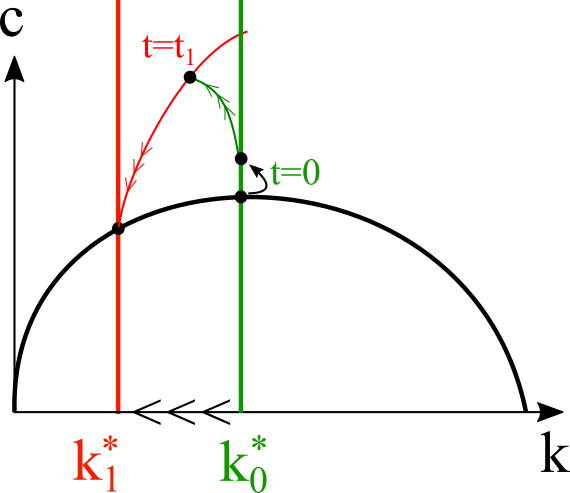
\includegraphics[width=0.8\textwidth]{3.a}



%%%%%%%%%%%%%%%%%
%     Part d    %
%%%%%%%%%%%%%%%%%
\newpage\problem{}{
    \begin{enumerate}[label=(\alph*)]
    \setcounter{enumi}{3}
    \item In light of your answers to parts (a), (b), and (c), what must $c$ do at time 0?
    \end{enumerate} 
}

It must change discontinuously in order to jump on a path that leads to the saddle path that it will be on at $t_1$.



%%%%%%%%%%%%%%%%%
%     Part e    %
%%%%%%%%%%%%%%%%%
\newpage\problem{}{
    \begin{enumerate}[label=(\alph*)]
    \setcounter{enumi}{4}
    \item Summarize your results by sketching the paths of $c$ and $k$ as functions of time.
    \end{enumerate} 
}


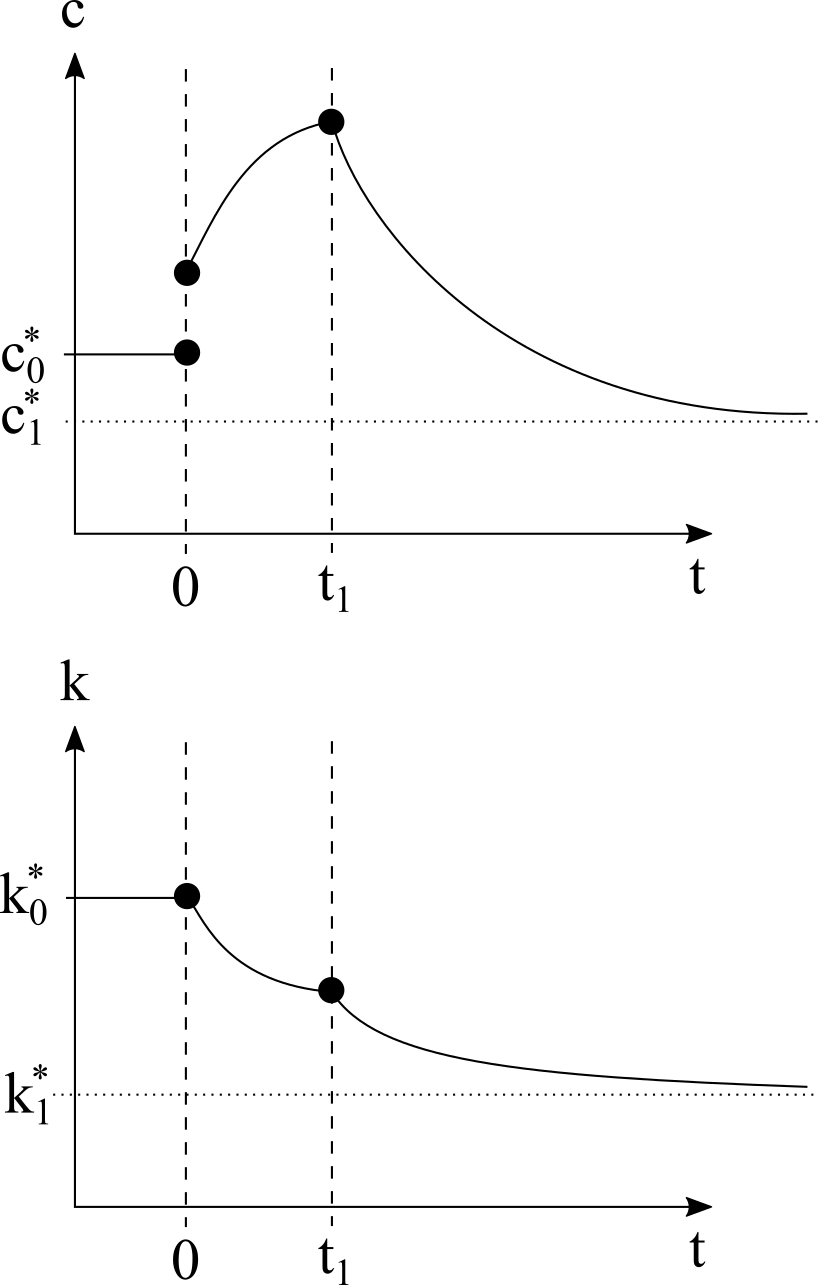
\includegraphics[width=0.6\textwidth]{3.e}



\end{document}

